\documentclass[addpoints]{exam}
\usepackage{amsfonts,amsmath,amsthm}
\usepackage{geometry}
\usepackage{hyperref}
\usepackage{titling}
\usepackage{tikz}
\usetikzlibrary{automata, positioning, arrows}
\tikzset{
  ->,  % makes the edges directed
  >=stealth, % makes the arrow heads bold
  node distance=2cm, % specifies the minimum distance between two nodes. 
  every state/.style={thick, fill=gray!10}, % sets the properties for each ’state’ node
  initial text=$ $, % sets the text that appears on the start arrow 
}
% Header and footer.
\pagestyle{headandfoot}
\runningheadrule
\runningfootrule
\runningheader{CS 212}{HW 1: Regular Languages}{Fall 2023}
\runningfooter{}{Page \thepage\ of \numpages}{}
\firstpageheader{}{}{}

\boxedpoints

\usepackage{draftwatermark}
\SetWatermarkText{Sample Solution}
\SetWatermarkScale{3}
\printanswers

\theoremstyle{claim}
\newtheorem{claim}{Claim}

\title{Homework 1: Regular Languages: Automata and Expressions}
\author{CS 212 Nature of Computation\\Habib University}
\date{Fall 2023}

\begin{document}
\maketitle

\section*{General instructions}
\begin{itemize}
\item For drawing finite automata, see  \href{https://www3.nd.edu/~kogge/courses/cse30151-fa17/Public/other/tikz_tutorial.pdf}{this TikZ guide} or \href{https://www.jflap.org}{the JFLAP tool}. Hand drawn diagrams will not be accepted.
\item Please ensure that your solutions are neatly formatted and organized, and use clear and
concise language.
\item Please consult Canvas for a rubric containing the breakdown of points for each problem.
\item For all the problems below, $\Sigma=\{a,b\}$.
\item Some of the problems below make use of the following count function.
\[
    n_a(w) =  \text{the number of occurences of } a\text{ in } w, \text{ where } a\in\Sigma,w\in\Sigma^*.
\]
\end{itemize}

\section*{Problems}
\begin{questions}

\question[15] List 2 members and 2 non-members of the language, $(a \cup ba \cup bb)\Sigma^*$.
  \begin{solution}
    Members: $ba, bb$\\
    Non-members: $\epsilon, b$\\
  \end{solution}
\question[20] Provide the state diagram of a simplified DFA that recognizes the language, 
  \[
    A=\{w\in\Sigma^* \mid n_a(w) \ge 2, n_b(w) \le 1\}.
  \]
  \begin{solution} The language can be expressed as: $aaa^* + baaa^* + abaa^* + aaa^*ba^*$.

    This helps to design the following NFA.
    
    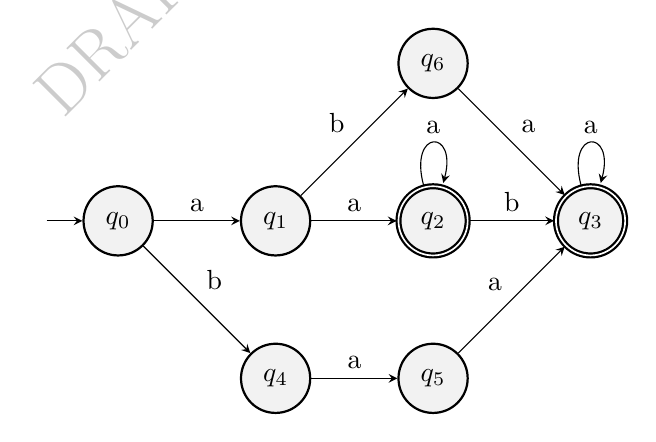
\begin{tikzpicture}
      \node[state, initial] (q0) {$q_0$};
      \node[state, right of=q0] (q1) {$q_1$};
      \node[state, accepting, right of=q1] (q2) {$q_2$};
      \node[state, accepting, right of=q2] (q3) {$q_3$};
      \node[state, below of=q1] (q4) {$q_4$};
      \node[state, right of=q4] (q5) {$q_5$};
      \node[state, above of=q2] (q6) {$q_6$};
      
      \draw
      (q0) edge[above] node{a} (q1)
      (q1) edge[above] node{a} (q2)
      (q2) edge[above] node{b} (q3)
      (q0) edge[above right] node{b} (q4)
      (q4) edge[above] node{a} (q5)
      (q5) edge[above left] node{a} (q3)
      (q1) edge[above left] node{b} (q6)
      (q6) edge[above right] node{a} (q3)
      (q2) edge[loop above] node{a} (q2)
      (q3) edge[loop above] node{a} (q3)
      ;
    \end{tikzpicture}

    Converting this NFA to a DFA results in a the addition of a \textit{dead} state, $q_7$.
    
    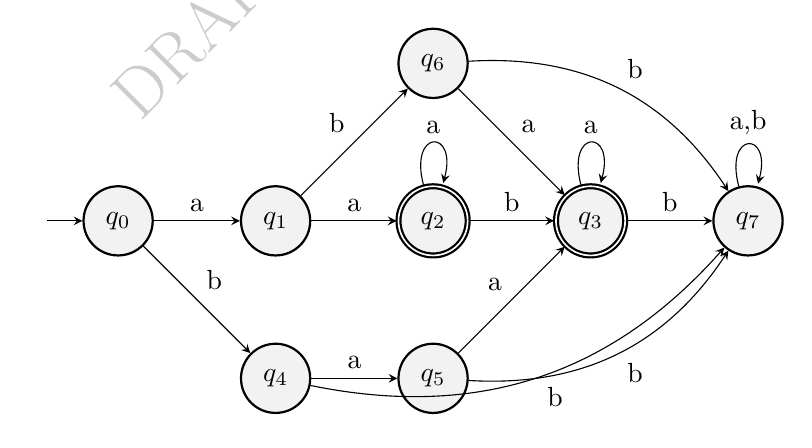
\begin{tikzpicture}
      \node[state, initial] (q0) {$q_0$};
      \node[state, right of=q0] (q1) {$q_1$};
      \node[state, accepting, right of=q1] (q2) {$q_2$};
      \node[state, accepting, right of=q2] (q3) {$q_3$};
      \node[state, below of=q1] (q4) {$q_4$};
      \node[state, right of=q4] (q5) {$q_5$};
      \node[state, above of=q2] (q6) {$q_6$};
      \node[state, right of=q3] (q7) {$q_7$};
      
      \draw
      (q0) edge[above] node{a} (q1)
      (q1) edge[above] node{a} (q2)
      (q2) edge[above] node{b} (q3)
      (q0) edge[above right] node{b} (q4)
      (q4) edge[above] node{a} (q5)
      (q5) edge[above left] node{a} (q3)
      (q1) edge[above left] node{b} (q6)
      (q6) edge[above right] node{a} (q3)
      (q2) edge[loop above] node{a} (q2)
      (q3) edge[loop above] node{a} (q3)
      (q3) edge[above] node{b} (q7)
      (q6) edge[bend left, above right] node{b} (q7)
      (q4) edge[bend right, below right] node{b} (q7)
      (q5) edge[bend right, below right] node{b} (q7)
      (q7) edge[loop above] node{a,b} (q7)
      ;
    \end{tikzpicture}
  \end{solution}

  
\question[30] Given the languages, $A$ and $B$, we derive the language, $C = \{ w\in A \mid w \in B \}$.

  Prove or disprove the following claim.
  \begin{claim}
    If $A$ and $B$ are regular languages, then so is $C$.
  \end{claim}
  
  \begin{solution}
    We prove the claim by referring to a construction described in our textbook.

    \begin{proof}
      We notice that $C = A \cap B$.

      The construction of the corresponding machine is described in footnote 3 in the proof of Theorem 1.25 in the textbook.
    \end{proof}
  \end{solution}
  
\question[35] Given the languages, $A$ and $B$, we define the following operation.
  \[
    A\smile_a B = \{ u\in A \mid \exists v\in B \ni n_a(u) = n_a(v) \}
  \]

  Prove or disprove the following claim.
  \begin{claim}
    The class of regular languages is closed under $\smile_a$.
  \end{claim}

  \begin{solution}
    We prove the claim by using the result in the previous question, i.e. closure of regular languages under intersection.

    \begin{proof}
    We notice that $A\smile_a B$ can be expressed as $A \cap B'$ where   
    \[
      B' = \{ u\in \Sigma^* \mid \exists v\in B \ni n_a(u) = n_a(v) \}.
    \]
    Given regular languages, $A$ and $B$, if $B'$ is regular then so is $A \cap B'$ or $A\smile_a B$.

    It remains to show that $B'$ is regular. We do so by deriving a regular expression for $B'$.

    The strings in $B'$ contain the same number of $a$s as the strings in $B$, and may contain an arbitrary number of $b$s. Given a string, $v$ in $B$, we can consider the following cases for a corresponding string, $u$, in $B'$. That is, $u$ contains the same number of $a$s as $v$.
    \begin{enumerate}
    \item $v$ contains $a$s: each $a$ in $v$ can be surrounded by 0 or more $b$s to obtain $u$.
    \item $v$ contains no $a$s and some $b$s: each $b$ in $v$ can be replaced with 0 or more $b$s to obtain $u$.
    \item $v$ contains no $a$s and no $b$s: $u$ contains 0 or more $b$s.
    \end{enumerate}

    The following table shows how a regular expression, $R'$, for $B'$ can be obtained from the regular expression. $R$, for $B$. It contains substitution rules to be applied to expressions in $R$ in order to obtain the corresponding expression in $R'$.

    \[
    \begin{array}{cc}
      R & R' \\
      \hline
      \emptyset & b^* \\
      \epsilon & b^* \\
      a & b^*ab^* \\
      b & b^* \\
      R_1\cup R_2 & R_1\cup R_2 \\
      R_1\circ R_2 & R_1\circ R_2 \\
      R_1^* & R_1^* \\
    \end{array}
    \]
    \end{proof}
    We note that the obtained grammar may leave a lot of room for simplification. That is not our concern here.
  \end{solution}
\end{questions}

\end{document}

%%% Local Variables:
%%% mode: latex
%%% TeX-master: t
%%% End:
